\documentclass{article}
\usepackage[utf8]{inputenc}

\title{CSE3500 — Programming Assignment 1}
\author{Mike Medved (mfm19005), Benny Chen (bec19009)}
\date{September 19th, 2022}

\usepackage{color}
\usepackage{amsmath,amsthm,amsfonts,amssymb,amscd}
\usepackage[margin=1in]{geometry} 
\usepackage{listings}
\usepackage{xcolor}
\usepackage{minted}
\usepackage{hyperref}
\usepackage{graphicx}

\hypersetup{
    colorlinks=true,
    linkcolor=blue,
    linkbordercolor={0 0 1}
}

\usemintedstyle{emacs}

\begin{document}

\maketitle

\subsection*{Recurrence Relation}

The below recurrence relation models the dynamic programming algorithm for this exercise to detect the lowest-energy horizontal seam of an image.

\begin{equation*}
    seam(j, i) = energy(j, i) + min \left(
    \begin{array}{lr}
        seam(j - 1, i - 1) \\
        seam(j - 1, i) \\
        seam(j - 1, if + 1)
    \end{array}
    \right)
\end{equation*}

\subsection*{Exponential Growth of Vertical Seam Complexity}

Given that $m > 1$, we can assume that the growth of possible vertical seams is exponential since our table must add another column. This will add another $m-i$ possibilities for each row $m$, and in turn would require the algorithm to recalculate the right-most possible seam for each row. This would cause a cascading effect down the table, and would result in an exponential complexity for the algorithm to compute the lowest-energy seam.

$\hfill \break$
In the case of this algorithm, this would come out to be $3^n$ since there are three possible directions at each step. This implementation of the algorithm only considers \textit{left}, \textit{right}, and \textit{down} as valid extensions of the seam, and as such there are $n$ seam extension coordinates spanning the height of the image to compute. 

\subsection*{Asymptotic Runtime}

The asymptotic runtime of our dynamic programming algorithm is $O(n^2)$ with an $n*m$ table, where $n$ and $m$ are the dimensions of the image. This is because we must iterate over every pixel of the image in order to fabricate the seam.


\begin{figure}[!htb]
    \minipage{0.5\textwidth}
        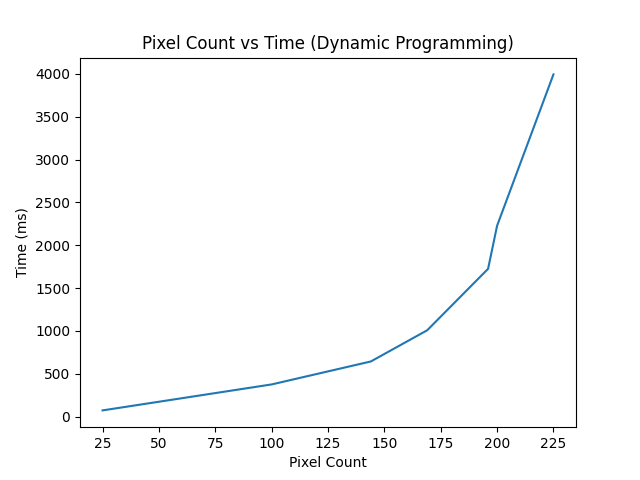
\includegraphics[width=\linewidth,height=6cm]{../benchmark/dp_runtimes.png}
        \label{fig:geometry}
        \caption{Dynamic Programming Runtimes} 
    \endminipage\hfill
    \minipage{0.5\textwidth}
        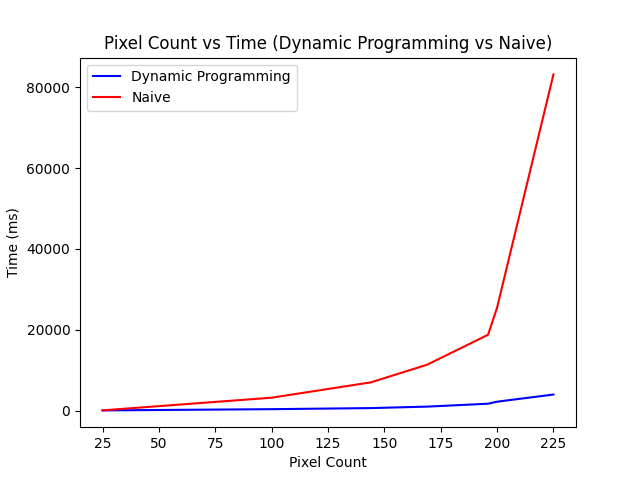
\includegraphics[width=\linewidth,height=6cm]{../benchmark/stacked_runtimes.png}
        \label{fig:golden_ratio}
        \caption{Dynamic Runtime vs Naive Runtime} 
\endminipage
\end{figure}

\newpage
\subsection*{Benchmarking Analysis}

The benchmarks we ran against our code make sense with respect to the intuition laid out for this exercise.

$\hfill \break$
The dynamic programming solution for this problem has a theoretical runtime of $O(n^2)$, which can be roughly seen in the generated plots above. Similarly, the runtime of our implementation of the naive solution is theoretically meant to be $O(n^3)$, which is also modelled in the generated plots above. 

$\hfill \break$
The runtime of the naive solution far less efficient than the runtime of the dynamic programming solution, which is expected since the naive solution is neither optimized, nor efficient. This is because the naive solution uses a brute-force approach to find the seam, and as such must iterate over every possible seam in order to find the lowest-energy seam.

$\hfill \break$
In this way, the dynamic programming solution is much more efficient than the naive solution, and as such is the preferred solution for this problem. Thus, we have demonstrated the vastly superior performance of the dynamic programming solution over the naive solution.

\end{document}
